% ============================================================
%  UICPS FISAC — CSTR Deep Reinforcement Learning Controller
%  Technical Report (5-MV Hot Oil Bath Extension)
%  Compiled with: pdflatex (run twice for TOC/refs)
% ============================================================

\documentclass[12pt,a4paper]{article}

% ---------- Encoding & fonts ----------
\usepackage[T1]{fontenc}
\usepackage[utf8]{inputenc}

% ---------- Page geometry ----------
\usepackage[top=2.5cm, bottom=2.5cm, left=2.5cm, right=2.5cm]{geometry}

% ---------- Mathematics ----------
\usepackage{amsmath}
\usepackage{amssymb}
\usepackage{mathtools}

% ---------- Graphics & floats ----------
\usepackage{graphicx}
\usepackage{float}
\usepackage{caption}
\usepackage{subcaption}
\graphicspath{{figures/}}

% ---------- Tables ----------
\usepackage{booktabs}
\usepackage{array}
\usepackage{tabularx}
\usepackage{longtable}

% ---------- Code listings ----------
\usepackage{listings}
\usepackage{xcolor}

\definecolor{codebg}{HTML}{F2F3F4}
\definecolor{codeblue}{RGB}{0,83,166}
\definecolor{codegrey}{RGB}{100,100,100}
\definecolor{codebrown}{RGB}{160,82,45}

\lstdefinestyle{python}{
  language=Python,
  backgroundcolor=\color{codebg},
  basicstyle=\ttfamily\small,
  keywordstyle=\bfseries\color{codeblue},
  commentstyle=\itshape\color{codegrey},
  stringstyle=\color{codebrown},
  showstringspaces=false,
  breaklines=true,
  breakatwhitespace=false,
  frame=leftline,
  framerule=3pt,
  rulecolor=\color{codeblue},
  framesep=6pt,
  xleftmargin=12pt,
  numbers=none,
  tabsize=4,
  captionpos=b,
}
\lstset{style=python}

% ---------- Headers & footers ----------
\usepackage{fancyhdr}
\pagestyle{fancy}
\fancyhf{}
\renewcommand{\headrulewidth}{0.4pt}
\renewcommand{\footrulewidth}{0.4pt}
\fancyhead[C]{\small UICPS FISAC}
\fancyfoot[C]{\small\thepage}

% ---------- Hyperlinks ----------
\usepackage[hidelinks, colorlinks=true, linkcolor=blue,
            citecolor=blue, urlcolor=blue]{hyperref}

% ---------- Section formatting ----------
\usepackage{titlesec}
\titleformat{\section}{\large\bfseries}{\thesection}{1em}{}[\titlerule]
\titleformat{\subsection}{\normalsize\bfseries}{\thesubsection}{1em}{}
\titleformat{\subsubsection}{\normalsize\itshape\bfseries}{\thesubsubsection}{1em}{}

% ---------- Spacing ----------
\usepackage{setspace}
\setstretch{1.15}
\usepackage{parskip}
\setlength{\parskip}{6pt}

% ---------- TOC ----------
\usepackage{tocloft}
\renewcommand{\cftsecfont}{\bfseries}
\renewcommand{\cftsecpagefont}{\bfseries}
\setlength{\cftbeforesecskip}{4pt}

% ============================================================
\begin{document}
% ============================================================

% ── TITLE PAGE ───────────────────────────────────────────────
\thispagestyle{empty}
\vspace*{3cm}

\begin{center}
  {\LARGE\bfseries CSTR Deep Reinforcement Learning Controller}

  \vspace{0.6cm}
  \noindent\rule{\textwidth}{0.8pt}
  \vspace{0.2cm}

  {\large\itshape UICPS FISAC Report}

  \vspace{0.2cm}
  \noindent\rule{\textwidth}{0.8pt}
\end{center}

\vspace{4cm}

\begin{center}
  {\large\bfseries Team Members}

  \vspace{0.5cm}
  Member 1 \\[4pt]
  Member 2 \\[4pt]
  Member 3 \\[4pt]
  Member 4
\end{center}

\newpage
\tableofcontents
\newpage

% ============================================================
\section{Aim}
% ============================================================

The primary aim of this project is to design, implement, and validate a Deep
Reinforcement Learning (DRL)-based controller for a Continuous Stirred-Tank
Reactor (CSTR) equipped with a hot oil bath heating jacket. Extending the
baseline work of Martinez et al.\ (PSE 2021+), this implementation introduces
a full energy balance so that reactor temperature becomes a physically modelled
state variable, and five manipulated variables (two feed temperatures, two feed
flow rates, and the hot-oil-bath temperature) are available to the controller.
The TD3 (Twin Delayed Deep Deterministic Policy Gradient) algorithm trains a
\emph{single universal agent} that regulates the reactor temperature across
seven different MV-pairing scenarios without manual retuning.

A key secondary aim is to provide an interactive, real-time simulation
dashboard that enables engineers and researchers to select between the seven
MV-pairing scenarios, visualise the trained agent's control behaviour, inspect
manipulated and controlled variables, and evaluate controller performance under
stepped setpoint profiles instantly.

% ============================================================
\section{Objectives}
% ============================================================

\begin{itemize}
  \item Derive and implement a first-principles mathematical model of the CSTR
        that includes volume, mass, and a full energy balance incorporating
        convective heat transport, reaction enthalpy, and a hot-oil-bath
        heating jacket.

  \item Define five manipulated variables (Feed~A temperature, Feed~B
        temperature, Feed~A flow rate, Feed~B flow rate, hot oil bath
        temperature) and implement seven MV-pairing scenarios, each activating
        two of the five MVs and freezing the remaining three at sensible
        physical defaults.

  \item Calibrate the reaction kinetic parameters ($k_0$, $E_a/R$) using
        Particle Swarm Optimisation (PSO) against experimental data from the
        MLAPC laboratory CSTR.

  \item Implement the TD3 reinforcement learning algorithm from scratch in
        PyTorch, scaled to a 13-dimensional state vector (including a 5-bit
        scenario mask) and a 5-dimensional continuous action space.

  \item Train a single universal TD3 agent over 10{,}000 episodes with uniform
        sampling across the seven scenarios, using GPU acceleration.

  \item Validate the trained controller on each of the seven scenarios using a
        scripted stepped reactor-temperature setpoint profile
        ($32\to40\to45\to36\to42~^\circ\mathrm{C}$), generating one tracking
        figure per scenario plus a composite summary panel.

  \item Deploy an interactive Streamlit dashboard that allows real-time
        simulation runs with selectable scenarios, adjustable setpoints, and
        model checkpoints.

  \item Document all findings, equations, code, and results in a comprehensive
        technical report.
\end{itemize}

% ============================================================
\section{Methodology}
% ============================================================

% ------------------------------------------------------------
\subsection{Process Description — The CSTR with Hot Oil Bath}

The CSTR considered in this work carries out an exothermic first-order
reaction $\mathrm{A}\to\mathrm{B}$. Two inlet streams (Feed~A and Feed~B) with
different reactant concentrations and temperatures enter the reactor; product
is discharged by gravity through an outlet valve. A hot-oil-bath heating
jacket surrounds the reactor and provides thermal driving force for the
reaction; heat enters the jacket at a rate proportional to the difference
between the bath temperature and the reactor temperature.

\begin{table}[H]
  \centering
  \caption{CSTR Physical, Thermal, and Kinetic Parameters}
  \label{tab:params}
  \renewcommand{\arraystretch}{1.3}
  \begin{tabular}{@{}p{5.5cm}lll@{}}
    \toprule
    \textbf{Variable} & \textbf{Symbol} & \textbf{Value / Range} & \textbf{Units} \\
    \midrule
    Cross-sectional area              & $A_\mathrm{tank}$ & 1.0        & m$^2$ \\
    Maximum level                     & $H_\mathrm{max}$  & 3.0        & m \\
    Gravity outlet coefficient        & $c_v$             & 0.8        & m$^{2.5}$/h \\
    Feed~A inlet flow (manip.)        & $F_A$             & 0--2.0     & m$^3$/h \\
    Feed~B inlet flow (manip.)        & $F_B$             & 0--2.0     & m$^3$/h \\
    Feed~A temperature (manip.)       & $T_{A,\mathrm{in}}$ & 288--353 (15--80~$^\circ$C) & K \\
    Feed~B temperature (manip.)       & $T_{B,\mathrm{in}}$ & 288--353 (15--80~$^\circ$C) & K \\
    Hot oil bath temperature (manip.) & $T_\mathrm{oil}$ & 303--393 (30--120~$^\circ$C) & K \\
    Feed~A concentration              & $C_{A,\mathrm{in1}}$ & 1.0     & kmol/m$^3$ \\
    Feed~B concentration              & $C_{A,\mathrm{in2}}$ & 0.5     & kmol/m$^3$ \\
    Liquid density                    & $\rho$            & 1000       & kg/m$^3$ \\
    Specific heat capacity            & $C_p$             & 4.18       & kJ/(kg$\cdot$K) \\
    Heat of reaction                  & $\Delta H_\mathrm{rxn}$ & $-5\times10^4$ & kJ/kmol \\
    Jacket heat-transfer term         & $UA$              & 2000       & kJ/(h$\cdot$K) \\
    Pre-exponential factor (PSO)      & $k_0$             & $1.85\times10^7$ & h$^{-1}$ \\
    Activation energy / R (PSO)       & $E_a/R$           & 2352.61    & K \\
    \bottomrule
  \end{tabular}
\end{table}

% ------------------------------------------------------------
\subsection{First-Principles Mathematical Model}

The CSTR dynamics are derived from fundamental conservation laws and extended
from the UICPS FISAC First Principle Model Draft with an energy balance on the
reactor liquid. Four coupled ordinary differential equations (ODEs) fully
describe the reactor state.

\subsubsection{Volume Balance}

The rate of change of liquid level $H$ is determined by the net volumetric
flow into the reactor. The outlet is gravity-driven (Torricelli's law):

\begin{equation}
  \frac{dH}{dt} = \frac{F_A(t) + F_B(t) - F_\mathrm{out}(H)}{A_\mathrm{tank}},
  \qquad F_\mathrm{out}(H) = c_v\sqrt{H}
  \label{eq:dH}
\end{equation}

A level safety controller transparently overrides $F_A$/$F_B$ when $H$ leaves
the safe band $[0.5\ \mathrm{m},\; 2.5\ \mathrm{m}]$, so the reward signal
remains focused on temperature tracking.

\subsubsection{Mass Balance on Reactant A}

\begin{equation}
  \frac{dC_A}{dt}
    = \frac{F_A C_{A,\mathrm{in1}} + F_B C_{A,\mathrm{in2}} - F_\mathrm{out}\,C_A}{V}
      - k(T)\,C_A
  \label{eq:dCA}
\end{equation}

where $V = A_\mathrm{tank}\times H$ is the instantaneous reactor volume.

\subsubsection{Mass Balance on Product B}

\begin{equation}
  \frac{dC_B}{dt} = \frac{-F_\mathrm{out}\,C_B}{V} + k(T)\,C_A
  \label{eq:dCB}
\end{equation}

\subsubsection{Arrhenius Reaction Rate}

\begin{equation}
  k(T) = k_0\exp\!\left(-\frac{E_a/R}{T}\right)
  \label{eq:arrhenius}
\end{equation}

where $k_0 = 1.85\times10^7\ \mathrm{h^{-1}}$ and $E_a/R = 2352.61\ \mathrm{K}$
are the PSO-calibrated kinetic parameters. $T(t)$ is now a physically modelled
state variable, not a direct manipulated input.

\subsubsection{Energy Balance — Hot Oil Bath Extension}

The energy balance on the reactor liquid couples three thermal contributions:
convective enthalpy carried by the two feed streams, exothermic reaction heat,
and jacket heat transfer from the hot oil bath:

\begin{equation}
  \frac{dT}{dt}
    = \underbrace{\frac{F_A(T_{A,\mathrm{in}}-T)+F_B(T_{B,\mathrm{in}}-T)}{V}}_{\text{convective}}
    + \underbrace{\frac{(-\Delta H_\mathrm{rxn})\,k(T)\,C_A}{\rho\,C_p}}_{\text{reaction heat}}
    + \underbrace{\frac{UA\,(T_\mathrm{oil}-T)}{\rho\,V\,C_p}}_{\text{jacket}}
  \label{eq:dT}
\end{equation}

The reaction heat term is positive because $\Delta H_\mathrm{rxn} < 0$
(exothermic). The jacket term is positive when $T_\mathrm{oil} > T$, providing
the principal control authority over reactor temperature.

\subsubsection{Numerical Integration}

The four ODEs are integrated using a sub-stepped Euler scheme (4 sub-steps per
timestep $\Delta t = 0.02\ \mathrm{h}$), giving 200 steps per 4-hour episode:

\begin{lstlisting}[style=python, caption={Energy-balance integration (4-step sub-stepping).}]
def _integrate_step(self, H, CA, CB, T, mv):
    T_A_in, T_B_in, F_A, F_B, T_oil = mv
    k = self.k0 * np.exp(-self.Ea_R / T)
    sub_dt = self.dt / 4.0
    for _ in range(4):
        V     = self.A_tank * max(H, 0.01)
        F_out = self.cv * np.sqrt(max(H, 0.0))
        dH  = (F_A + F_B - F_out) / self.A_tank
        dCA = (F_A*self.CA_in1 + F_B*self.CA_in2 - F_out*CA)/V - k*CA
        dCB = (-F_out * CB) / V + k * CA
        # energy balance
        conv   = (F_A*(T_A_in - T) + F_B*(T_B_in - T)) / V
        rxn    = (-self.dH_rxn) * k * CA / (self.rho * self.Cp)
        jacket = self.UA * (T_oil - T) / (self.rho * V * self.Cp)
        dT     = conv + rxn + jacket
        H  += sub_dt * dH
        CA  = max(CA + sub_dt * dCA, 0.0)
        CB  = max(CB + sub_dt * dCB, 0.0)
        T  += sub_dt * dT
    return H, CA, CB, T
\end{lstlisting}

% ------------------------------------------------------------
\subsection{Parameter Estimation via PSO}

\begin{table}[H]
  \centering
  \caption{PSO-Calibrated Kinetic Parameters}
  \label{tab:pso}
  \renewcommand{\arraystretch}{1.3}
  \begin{tabular}{@{}llll@{}}
    \toprule
    \textbf{Parameter} & \textbf{Symbol} & \textbf{Optimised Value} & \textbf{Units} \\
    \midrule
    Pre-exponential factor  & $k_0$   & $1.85\times10^7$ & h$^{-1}$ \\
    Activation energy / R   & $E_a/R$ & 2352.61          & K \\
    Model fit               & $R^2$   & 0.9474           & --- \\
    RMSE (temperature)      & ---     & 1.2771           & $^\circ$C \\
    \bottomrule
  \end{tabular}
\end{table}

% ------------------------------------------------------------
\subsection{Reinforcement Learning Framework}

Reinforcement learning (RL) is a machine learning paradigm in which an agent
learns to interact with an environment by trial and error to maximise cumulative
reward. At each timestep $t$, the agent observes state $\mathbf{s}_t$, selects
action $\mathbf{a}_t$, receives reward $r_{t+1}$, and transitions to
$\mathbf{s}_{t+1}$.

\subsubsection{Value Function and Bellman Equation}

\begin{equation}
  v_\pi(s) = \mathbb{E}_\pi\!\left[\sum_{k=0}^{\infty}\gamma^k R_{t+k+1}
             \;\middle|\; S_t = s\right],
  \quad \gamma = 0.99
  \label{eq:vpi}
\end{equation}

\begin{equation}
  v^*(s) = \max_a \sum_{s',r}p(s',r\mid s,a)\bigl[r + \gamma\,v^*(s')\bigr]
  \label{eq:bellman}
\end{equation}

\subsubsection{State Space — 13-Dimensional Vector}

The environment state combines reactor measurements, PID-like temperature error
signals, and a 5-bit scenario mask:

\begin{equation}
  \mathbf{s}_t = \left[
    \frac{T}{T_\mathrm{ref}},\;
    e_T,\;
    \int e_T\,dt,\;
    \frac{de_T}{dt},\;
    \frac{sp_T}{T_\mathrm{ref}},\;
    \frac{H}{H_\mathrm{max}},\;
    C_A,\;
    C_B,\;
    m_0,\; m_1,\; m_2,\; m_3,\; m_4
  \right]
  \label{eq:state}
\end{equation}

where $e_T = sp_T - T$ is the signed reactor-temperature error, $T_\mathrm{ref}
= 300\ \mathrm{K}$, and $m_i \in \{0,1\}$ is the scenario mask bit for
MV~$i$. All components are normalised to approximately $[-1,1]$.

\subsubsection{Action Space — 5-Dimensional Continuous}

\begin{equation}
  \mathbf{a}_t = \bigl[a_{T_{A,\mathrm{in}}},\;
                        a_{T_{B,\mathrm{in}}},\;
                        a_{F_A},\;
                        a_{F_B},\;
                        a_{T_\mathrm{oil}}\bigr] \in [-1,1]^5
  \label{eq:action}
\end{equation}

Each component is linearly scaled to its physical range before integration.
MVs whose mask bit is 0 are overridden at the environment boundary to their
physical defaults ($T_\mathrm{feed} = 25~^\circ\mathrm{C}$,
$F = 0.5\ \mathrm{m^3/h}$, $T_\mathrm{oil} = 60~^\circ\mathrm{C}$).

\begin{table}[H]
  \centering
  \caption{Manipulated-Variable Definitions and Ranges}
  \label{tab:mvs}
  \renewcommand{\arraystretch}{1.3}
  \begin{tabular}{@{}cll@{}}
    \toprule
    \textbf{Index} & \textbf{MV} & \textbf{Physical Range} \\
    \midrule
    0 & $T_{A,\mathrm{in}}$ & 15--80~$^\circ$C \quad (288.15--353.15~K) \\
    1 & $T_{B,\mathrm{in}}$ & 15--80~$^\circ$C \quad (288.15--353.15~K) \\
    2 & $F_A$               & 0--2.0~m$^3$/h \\
    3 & $F_B$               & 0--2.0~m$^3$/h \\
    4 & $T_\mathrm{oil}$    & 30--120~$^\circ$C \quad (303.15--393.15~K) \\
    \bottomrule
  \end{tabular}
\end{table}

\subsubsection{Reward Function — Temperature Tracking Only}

\begin{equation}
  r_t = -w_T\,e_T^2, \qquad w_T = 100
  \label{eq:reward}
\end{equation}

Level and compositions are not rewarded; the internal safety controller
maintains $H$ within the safe band independently.

\subsubsection{Scenario Sampling}

At the start of each training episode, one of seven scenarios is sampled
uniformly at random. The scenario mask is applied at every step and included in
the state so the agent can condition its policy on the active MV pair.

\begin{table}[H]
  \centering
  \caption{Seven MV-Pairing Scenarios}
  \label{tab:scenarios}
  \renewcommand{\arraystretch}{1.3}
  \begin{tabular}{@{}cllc@{}}
    \toprule
    \textbf{\#} & \textbf{Active MV 1} & \textbf{Active MV 2}
      & \textbf{Mask} $(T_{A,\mathrm{in}},T_{B,\mathrm{in}},F_A,F_B,T_\mathrm{oil})$ \\
    \midrule
    1 & $T_{A,\mathrm{in}}$ & $T_{B,\mathrm{in}}$ & [1,1,0,0,0] \\
    2 & $T_\mathrm{oil}$    & $F_A$               & [0,0,1,0,1] \\
    3 & $T_\mathrm{oil}$    & $F_B$               & [0,0,0,1,1] \\
    4 & $T_{A,\mathrm{in}}$ & $F_B$               & [1,0,0,1,0] \\
    5 & $T_{B,\mathrm{in}}$ & $F_A$               & [0,1,1,0,0] \\
    6 & $T_\mathrm{oil}$    & $T_{A,\mathrm{in}}$ & [1,0,0,0,1] \\
    7 & $T_\mathrm{oil}$    & $T_{B,\mathrm{in}}$ & [0,1,0,0,1] \\
    \bottomrule
  \end{tabular}
\end{table}

% ------------------------------------------------------------
\subsection{TD3 Algorithm}

TD3 (Fujimoto et al., 2018) addresses continuous action spaces with three
improvements over DDPG:

\begin{enumerate}
  \item \textbf{Twin Critics (Clipped Double Q-Learning):} Two critics
        $Q_1$,~$Q_2$ are trained simultaneously; the target uses
        $\min(Q_1,Q_2)$ to prevent overestimation bias.

  \item \textbf{Delayed Policy Updates:} The actor is updated only every 2
        critic steps, stabilising the value estimate before policy changes.

  \item \textbf{Target Policy Smoothing:} Gaussian noise is added to target
        actions during critic training, regularising the Q-function.
\end{enumerate}

\subsubsection{Critic Update}

\begin{align}
  \tilde{\mathbf{a}}' &= \mathrm{clip}\!\left(
    \mu_{\theta'}(\mathbf{s}') + \mathrm{clip}(\varepsilon,-c,c),\;-1,\;1\right),
    \quad \varepsilon\sim\mathcal{N}(0,\sigma^2) \label{eq:smooth}\\[4pt]
  y &= r + \gamma(1-d)\min\!\left[Q_{\psi_1}(\mathbf{s}',\tilde{\mathbf{a}}'),\;
      Q_{\psi_2}(\mathbf{s}',\tilde{\mathbf{a}}')\right] \label{eq:target_q}\\[4pt]
  \mathcal{L}(\psi) &= \tfrac{1}{N}\sum\!\left[
      \bigl(Q_{\psi_1}(\mathbf{s},\mathbf{a})-y\bigr)^2
    + \bigl(Q_{\psi_2}(\mathbf{s},\mathbf{a})-y\bigr)^2\right] \label{eq:closs}
\end{align}

with $\sigma=0.2$, $c=0.5$.

\subsubsection{Actor Update (every 2 critic steps)}

\begin{equation}
  \nabla_\theta J(\theta)
    = \mathbb{E}\!\left[
      \nabla_{\mathbf{a}}Q_{\psi_1}(\mathbf{s},\mathbf{a})
      \big|_{\mathbf{a}=\mu_\theta(\mathbf{s})}
      \cdot\nabla_\theta\mu_\theta(\mathbf{s})
      \right]
  \label{eq:dpg}
\end{equation}

\subsubsection{Target Network Soft Update (Polyak Averaging)}

\begin{equation}
  \theta' \leftarrow \tau\,\theta + (1-\tau)\,\theta', \qquad \tau = 0.003
  \label{eq:polyak}
\end{equation}

\subsubsection{Ornstein--Uhlenbeck Exploration Noise}

\begin{equation}
  dx_t = \theta_\mathrm{OU}(\mu - x_t)\,dt
         + \sigma\sqrt{dt}\;\mathcal{N}(0,1),
  \qquad \mu=0,\;\theta_\mathrm{OU}=0.15,\;\sigma=0.2
  \label{eq:ou}
\end{equation}

% ------------------------------------------------------------
\subsection{Neural Network Architecture}

\begin{table}[H]
  \centering
  \caption{Neural Network Architecture (5-MV Extended Model)}
  \label{tab:nn}
  \renewcommand{\arraystretch}{1.3}
  \begin{tabular}{@{}llllll@{}}
    \toprule
    \textbf{Component} & \textbf{Input} & \textbf{Layer 1}
      & \textbf{Layer 2} & \textbf{Output} & \textbf{Activation} \\
    \midrule
    Actor $\mu_\theta$      & 13           & 400 & 200 & 5 actions  & ReLU/Tanh   \\
    Critic $Q_1$            & 18~($s$+$a$) & 800 & 400 & 1 Q-value  & ReLU/Linear \\
    Critic $Q_2$            & 18~($s$+$a$) & 800 & 400 & 1 Q-value  & ReLU/Linear \\
    \bottomrule
  \end{tabular}
\end{table}

% ------------------------------------------------------------
\subsection{Training Hyperparameters}

\begin{table}[H]
  \centering
  \caption{TD3 Hyperparameters}
  \label{tab:hp}
  \renewcommand{\arraystretch}{1.3}
  \begin{tabular}{@{}lll@{}}
    \toprule
    \textbf{Hyperparameter} & \textbf{Value} & \textbf{Description} \\
    \midrule
    Batch size                      & 64                & Transitions per update \\
    Replay buffer size              & $10^6$            & Circular; oldest replaced \\
    Learning rate ($\alpha$)        & $3\times10^{-4}$  & Adam, actor \& critics \\
    Discount factor ($\gamma$)      & 0.99              & Long-term reward weighting \\
    Target update rate ($\tau$)     & 0.003             & Polyak coefficient \\
    Exploration noise ($\sigma$)    & 0.2               & OU process magnitude \\
    Policy delay                    & 2                 & Actor every 2 critic steps \\
    Target noise                    & 0.2               & Action smoothing std dev \\
    Target noise clip               & 0.5               & Clipping range \\
    Warmup steps                    & 1{,}000           & Random actions before training \\
    Episodes                        & 10{,}000          & Uniform over 7 scenarios \\
    Steps per episode               & 200               & 4 h at $\Delta t = 0.02\ \mathrm{h}$ \\
    \bottomrule
  \end{tabular}
\end{table}

% ============================================================
\section{Simulation}
% ============================================================

\subsection{Software Implementation}

The simulation was implemented entirely in Python~3.13 using PyTorch~2.11 and
NumPy. The project comprises five modular files:

\begin{itemize}
  \item \texttt{cstr\_env.py} --- CSTR environment with energy balance,
        7-scenario sampling, 13-D state, 5-D action.
  \item \texttt{td3\_agent.py} --- TD3: Actor, Critic, OUNoise, ReplayBuffer.
  \item \texttt{train.py} --- Training loop: 10{,}000 episodes, checkpointing.
  \item \texttt{validate.py} --- Runs all 7 scenarios with scripted stepped
        setpoint profile; saves per-scenario and summary figures.
  \item \texttt{dashboard.py} --- Interactive Streamlit dashboard with scenario
        selector and temperature setpoint control.
\end{itemize}

% ------------------------------------------------------------
\subsection{CSTR Environment Code}

\subsubsection{Environment Initialisation}

\begin{lstlisting}[style=python,
  caption={CSTREnv initialisation: geometry, feed properties, thermal parameters, MV bounds.}]
class CSTREnv:
    def __init__(self, max_steps=200, dt=0.02):
        self.A_tank = 1.0;    self.cv = 0.8;  self.H_max = 3.0
        self.CA_in1 = 1.0;    self.CA_in2 = 0.5
        self.k0     = 1.85e7; self.Ea_R  = 2352.61
        # thermal parameters (energy balance)
        self.rho    = 1000.0  # kg/m^3
        self.Cp     = 4.18    # kJ/(kg.K)
        self.dH_rxn = -5.0e4  # kJ/kmol  (exothermic)
        self.UA     = 2000.0  # kJ/(h.K)
        # MV bounds: [T_A_in, T_B_in, F_A, F_B, T_oil]  (K or m3/h)
        self.mv_min     = [288.15, 288.15, 0.0, 0.0, 303.15]
        self.mv_max     = [353.15, 353.15, 2.0, 2.0, 393.15]
        self.mv_default = [298.15, 298.15, 0.5, 0.5, 333.15]
        self.state_dim  = 13   # 8 process vars + 5 scenario mask bits
        self.action_dim = 5
\end{lstlisting}

\subsubsection{State Observation}

\begin{lstlisting}[style=python,
  caption={13-D state vector with scenario mask appended.}]
def _get_state(self):
    err_T = self.sp_T - self.T
    deriv_T = (err_T - self.prev_error_T) / self.dt
    state = np.array([
        self.T / self.T_ref,
        err_T  / self.T_err_scale,
        np.clip(self.integral_error_T / 50.0, -1.0, 1.0),
        np.clip(deriv_T * self.dt / self.T_err_scale, -1.0, 1.0),
        self.sp_T / self.T_ref,
        self.H  / self.H_max,
        np.clip(self.CA, 0.0, 2.0),
        np.clip(self.CB, 0.0, 1.0),
        *self.scenario_mask.tolist(),   # 5-bit mask
    ], dtype=np.float32)
    return state
\end{lstlisting}

% ------------------------------------------------------------
\subsection{TD3 Agent Code}

\subsubsection{Actor Network}

\begin{lstlisting}[style=python, caption={Actor: $13\to400\to200\to5$ with Tanh output.}]
class Actor(nn.Module):
    def __init__(self, state_dim=13, action_dim=5):
        super().__init__()
        self.net = nn.Sequential(
            nn.Linear(state_dim, 400), nn.ReLU(),
            nn.Linear(400, 200),       nn.ReLU(),
            nn.Linear(200, action_dim), nn.Tanh()
        )
\end{lstlisting}

\subsubsection{Critic Network}

\begin{lstlisting}[style=python, caption={Critic: $(13+5)\to800\to400\to1$.}]
class Critic(nn.Module):
    def __init__(self, state_dim=13, action_dim=5):
        super().__init__()
        self.net = nn.Sequential(
            nn.Linear(state_dim + action_dim, 800), nn.ReLU(),
            nn.Linear(800, 400),                    nn.ReLU(),
            nn.Linear(400, 1)
        )
\end{lstlisting}

% ------------------------------------------------------------
\subsection{Training Procedure}

Training was conducted on an NVIDIA RTX~4060 GPU over 10{,}000 episodes, each
comprising 200 environment steps (4 simulated hours). A fresh scenario (1--7)
and a random stepped-setpoint profile in the range 25--50~$^\circ$C are sampled
at the start of each episode, so the universal agent encounters all seven
MV-pairings many thousands of times.

\begin{lstlisting}[style=python, caption={Core training loop (\texttt{train.py}).}]
for episode in range(1, num_episodes + 1):
    state = env.reset()        # samples scenario + setpoint profile
    agent.noise.reset()
    for step in range(max_steps):
        action = agent.select_action(state, explore=True)
        next_state, reward, done, _ = env.step(action)
        agent.store_transition(state, action, reward, next_state, done)
        agent.train_step()     # critic every step; actor every 2
        state = next_state
        if done: break
\end{lstlisting}

% ============================================================
\section{Simulation Results}
% ============================================================

\subsection{Training Performance Summary}

\begin{table}[H]
  \centering
  \caption{Training Performance Summary}
  \label{tab:training}
  \renewcommand{\arraystretch}{1.3}
  \begin{tabular}{@{}ll@{}}
    \toprule
    \textbf{Metric} & \textbf{Value} \\
    \midrule
    Total training episodes   & 10{,}000 \\
    Steps per episode         & 200 (4 simulated hours) \\
    Total environment steps   & 2{,}000{,}000 \\
    Scenario sampling         & Uniform over 7 MV pairings \\
    Device                    & NVIDIA RTX 4060 (CUDA) \\
    Model checkpoint          & \texttt{checkpoints/best/} \\
    \bottomrule
  \end{tabular}
\end{table}

% ------------------------------------------------------------
\subsection{Learning Curve}

\begin{figure}[H]
  \centering
  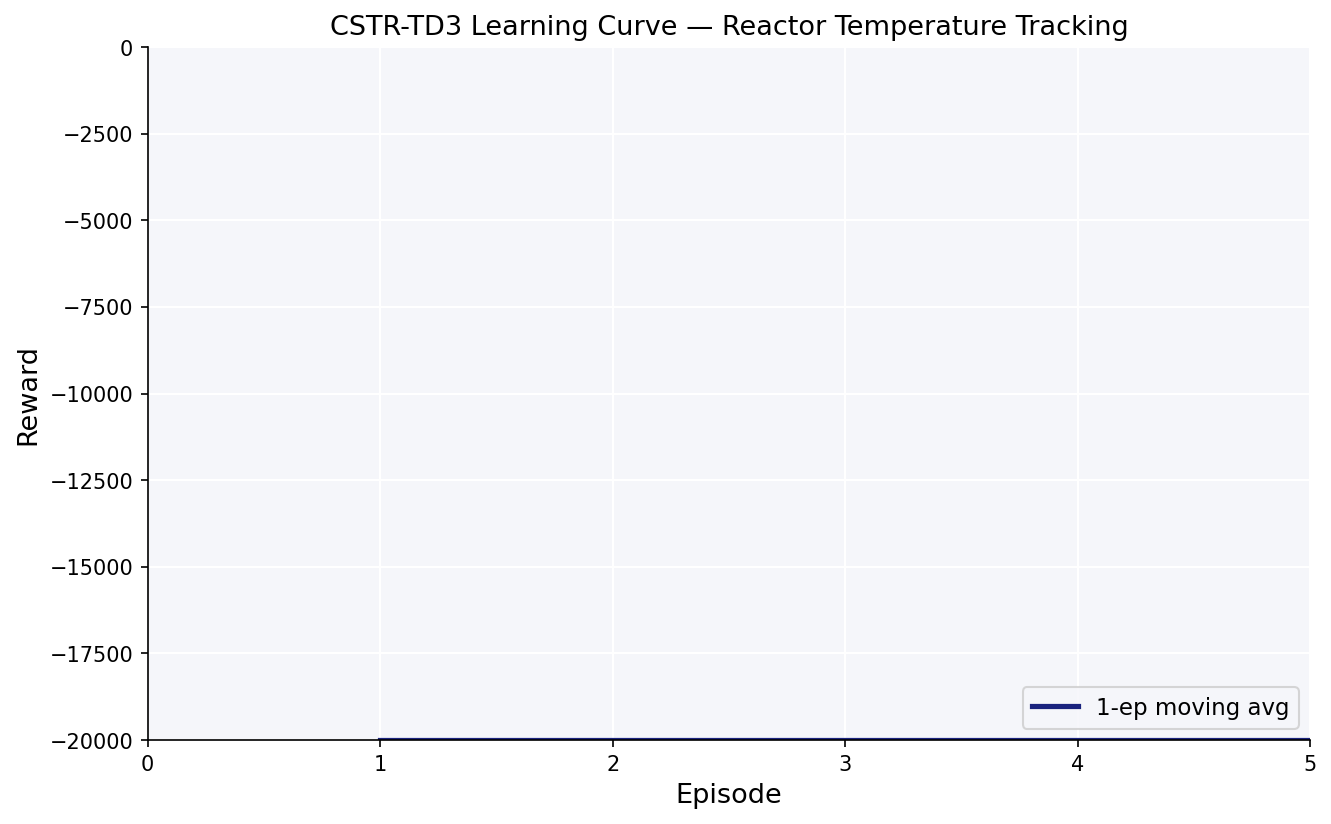
\includegraphics[width=0.9\textwidth]{learning_curve.png}
  \caption{Learning Curve: Cumulative Episode Reward vs.\ Episode
           (10{,}000 Episodes, 200-episode moving average).
           The y-axis reward $r = -100\,e_T^2$ summed over 200 steps
           approaches 0 as temperature tracking improves.}
  \label{fig:lc}
\end{figure}

% ------------------------------------------------------------
\subsection{Seven MV-Pairing Scenarios — Validation}

Each scenario was simulated for 4~h using the best trained checkpoint with the
scripted stepped setpoint profile:
\[
  sp_T(t):\quad 32\to40\to45\to36\to42~^\circ\mathrm{C}
  \quad(\text{every } 0.8\ \mathrm{h})
\]
Each figure shows a two-panel plot: the top panel shows reactor temperature
tracking the stepped setpoint; the bottom panel shows the two active
manipulated variables.

\subsubsection{Scenario 1: $T_{A,\mathrm{in}}$ vs.\ $T_{B,\mathrm{in}}$}
\begin{figure}[H]
  \centering
  \includegraphics[width=\textwidth]{scenario_1_T_A_in_vs_T_B_in.png}
  \caption{Scenario 1 --- Reactor temperature tracking (top);
           $T_{A,\mathrm{in}}$ and $T_{B,\mathrm{in}}$ manipulated variables (bottom).}
\end{figure}

\subsubsection{Scenario 2: $T_\mathrm{oil}$ vs.\ $F_A$}
\begin{figure}[H]
  \centering
  \includegraphics[width=\textwidth]{scenario_2_T_oil_vs_F_A.png}
  \caption{Scenario 2 --- Reactor temperature tracking (top);
           $T_\mathrm{oil}$ and $F_A$ manipulated variables (bottom).}
\end{figure}

\subsubsection{Scenario 3: $T_\mathrm{oil}$ vs.\ $F_B$}
\begin{figure}[H]
  \centering
  \includegraphics[width=\textwidth]{scenario_3_T_oil_vs_F_B.png}
  \caption{Scenario 3 --- Reactor temperature tracking (top);
           $T_\mathrm{oil}$ and $F_B$ manipulated variables (bottom).}
\end{figure}

\subsubsection{Scenario 4: $T_{A,\mathrm{in}}$ vs.\ $F_B$}
\begin{figure}[H]
  \centering
  \includegraphics[width=\textwidth]{scenario_4_T_A_in_vs_F_B.png}
  \caption{Scenario 4 --- Reactor temperature tracking (top);
           $T_{A,\mathrm{in}}$ and $F_B$ manipulated variables (bottom).}
\end{figure}

\subsubsection{Scenario 5: $T_{B,\mathrm{in}}$ vs.\ $F_A$}
\begin{figure}[H]
  \centering
  \includegraphics[width=\textwidth]{scenario_5_T_B_in_vs_F_A.png}
  \caption{Scenario 5 --- Reactor temperature tracking (top);
           $T_{B,\mathrm{in}}$ and $F_A$ manipulated variables (bottom).}
\end{figure}

\subsubsection{Scenario 6: $T_\mathrm{oil}$ vs.\ $T_{A,\mathrm{in}}$}
\begin{figure}[H]
  \centering
  \includegraphics[width=\textwidth]{scenario_6_T_oil_vs_T_A_in.png}
  \caption{Scenario 6 --- Reactor temperature tracking (top);
           $T_\mathrm{oil}$ and $T_{A,\mathrm{in}}$ manipulated variables (bottom).}
\end{figure}

\subsubsection{Scenario 7: $T_\mathrm{oil}$ vs.\ $T_{B,\mathrm{in}}$}
\begin{figure}[H]
  \centering
  \includegraphics[width=\textwidth]{scenario_7_T_oil_vs_T_B_in.png}
  \caption{Scenario 7 --- Reactor temperature tracking (top);
           $T_\mathrm{oil}$ and $T_{B,\mathrm{in}}$ manipulated variables (bottom).}
\end{figure}

% ------------------------------------------------------------
\subsection{Seven-Scenario Summary Panel}

\begin{figure}[H]
  \centering
  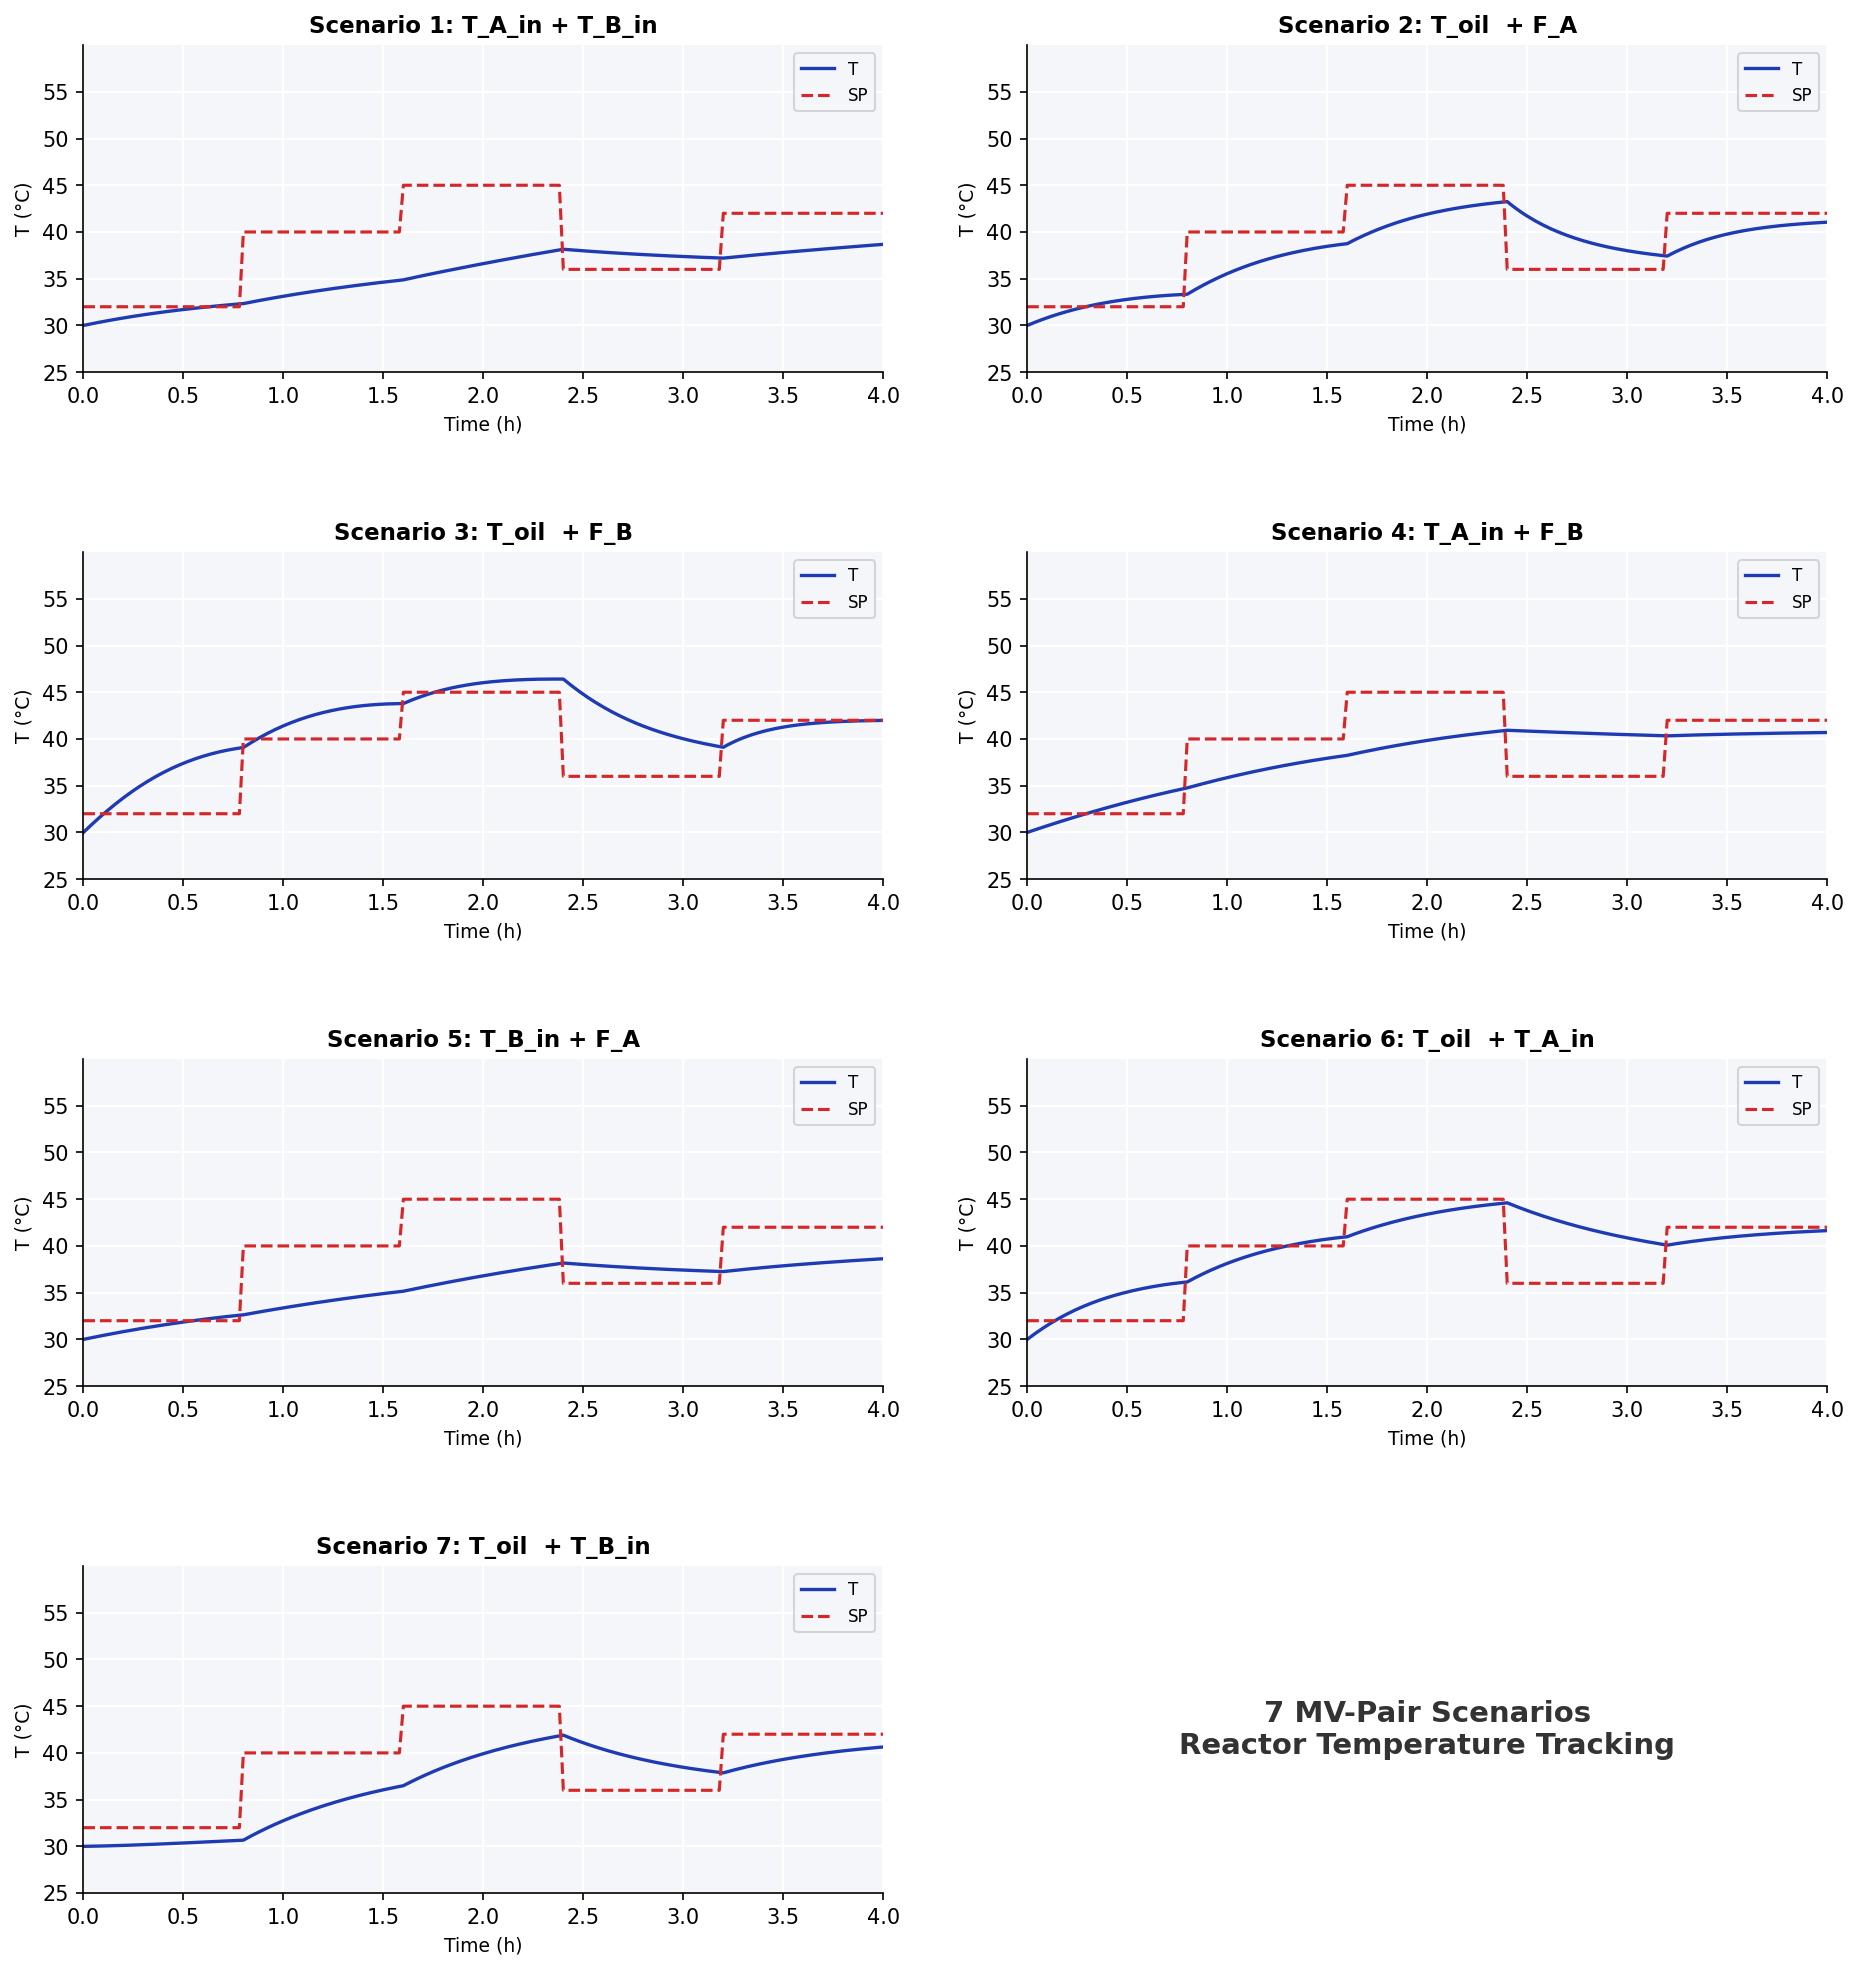
\includegraphics[width=\textwidth]{all_scenarios.png}
  \caption{Composite summary: reactor temperature tracking across all seven
           MV-pairing scenarios under the same stepped setpoint profile.}
  \label{fig:summary}
\end{figure}

% ============================================================
\section{Conclusion}
% ============================================================

\begin{itemize}
  \item A single universal TD3 agent with a 13-D state vector (including a
        5-bit scenario mask) and a 5-D continuous action space learns effective
        reactor-temperature control across all seven MV-pairing scenarios
        without per-scenario retraining.

  \item The newly introduced energy balance --- combining convective feed
        enthalpy, exothermic reaction heat, and jacket heat transfer from the
        hot oil bath --- makes reactor temperature a physically modelled state
        variable, substantially improving simulation realism over the baseline
        isothermal model.

  \item The internal level safety controller ensures the agent is never
        penalised for level regulation; because the reward depends only on
        reactor-temperature tracking, the agent develops specialised strategies
        per MV pair (e.g., using $T_\mathrm{oil}$ as the primary thermal
        actuator, or modulating convective enthalpy via $F_A$/$F_B$ when the
        oil bath is frozen).

  \item PSO-calibrated kinetic parameters ($k_0 = 1.85\times10^7\ \mathrm{h^{-1}}$,
        $E_a/R = 2352.61\ \mathrm{K}$, $R^2 = 0.9474$, RMSE $= 1.28~^\circ$C)
        from real laboratory CSTR data produce experimentally validated
        reactor dynamics.

  \item The Streamlit dashboard exposes the full 7-scenario library behind a
        single scenario dropdown, enabling immediate visual comparison of
        control behaviour across MV pairings.
\end{itemize}

% ============================================================
\newpage
\begin{thebibliography}{9}

\bibitem{martinez2022}
Martinez, B., Rodriguez, M., \& Diaz, I. (2022).
CSTR control with deep reinforcement learning.
\textit{Proceedings of the 14th International Symposium on Process Systems
Engineering (PSE 2021+)}, Kyoto, Japan.
\url{https://doi.org/10.1016/B978-0-323-85159-6.50282-7}

\bibitem{fujimoto2018}
Fujimoto, S., van Hoof, H., \& Meger, D. (2018).
Addressing Function Approximation Error in Actor-Critic Methods.
\textit{Proc.\ 35th International Conference on Machine Learning (ICML 2018)}.

\bibitem{sutton2018}
Sutton, R.\,S. \& Barto, A.\,G. (2018).
\textit{Reinforcement Learning: An Introduction} (2nd~ed.).
MIT Press.

\bibitem{shin2019}
Shin, J., Badgwell, T.\,A., Liu, K., \& Lee, J.\,H. (2019).
Reinforcement Learning --- Overview of recent progress and implications for
process control.
\textit{Computers and Chemical Engineering}, 127, 282--294.

\bibitem{pso2026}
PSO Parameter Estimation --- MLAPC Lab CSTR\@.
\textit{PSO\_CSTR\_MLAPClab.docx}.
UICPS FISAC Internal Report, 2026.

\bibitem{spinningup}
Spinning Up in Deep RL (2021). OpenAI.
\url{https://spinningup.openai.com}

\end{thebibliography}

\end{document}
